\hypertarget{syncprims-pmsm_8h}{\section{/home/roger/\-Net\-Beans\-Projects/log4cplus/include/log4cplus/thread/impl/syncprims-\/pmsm.h File Reference}
\label{syncprims-pmsm_8h}\index{/home/roger/\-Net\-Beans\-Projects/log4cplus/include/log4cplus/thread/impl/syncprims-\/pmsm.\-h@{/home/roger/\-Net\-Beans\-Projects/log4cplus/include/log4cplus/thread/impl/syncprims-\/pmsm.\-h}}
}
This graph shows which files directly or indirectly include this file\-:
\nopagebreak
\begin{figure}[H]
\begin{center}
\leavevmode
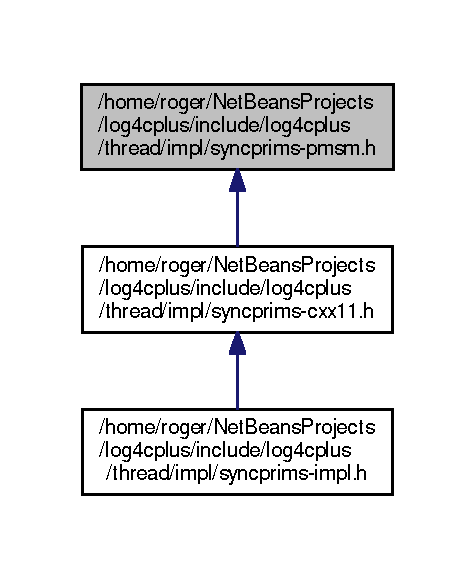
\includegraphics[width=228pt]{syncprims-pmsm_8h__dep__incl}
\end{center}
\end{figure}


\subsection{Detailed Description}
This file contains implementations of reader-\/writer locking primitive using other primitives, I\-O\-W poor man's rwlock. It does not contain any include guards because it is only a fragment to be included by syncprims-\/\{pthreads,win32\}.h. 